\chapter[Protótipos]{Protótipos}

\section{Baixa Fidelidade}

Os protótipos de baixa fidelidade foram concebidos durante a fase inicial do projeto. Desenhados à mão utilizando lápis, borracha e papel, foram feitas representações de maneira rápida e superficial, apenas margeando a ideia do projeto e definindo inicialmente sua interação com o usuário, não se preocupando tanto com elementos de layout, cores, disposições, etc.

\textbf{Telas:}

\section{Média Fidelidade}

Os protótipos de média fidelidade foram desenvolvidos apos a aplicação dos testes com os protótipos de baixa fidelidade. Utilizamos o softwares de prototipação Balsamiq para auxilio na apresentação da estrutura e o conteúdo da interface, definindo peso, relevância e relação dos elementos, formando o layout básico do projeto.

\textbf{Telas:}

\begin{figure}[H]
	\begin{adjustbox}{
		addcode={
			\begin{minipage}{
				\width}}{
					\caption{Protótipo Média Fidelidade}
					\end{minipage}
				},
				rotate=90,center
			}
    	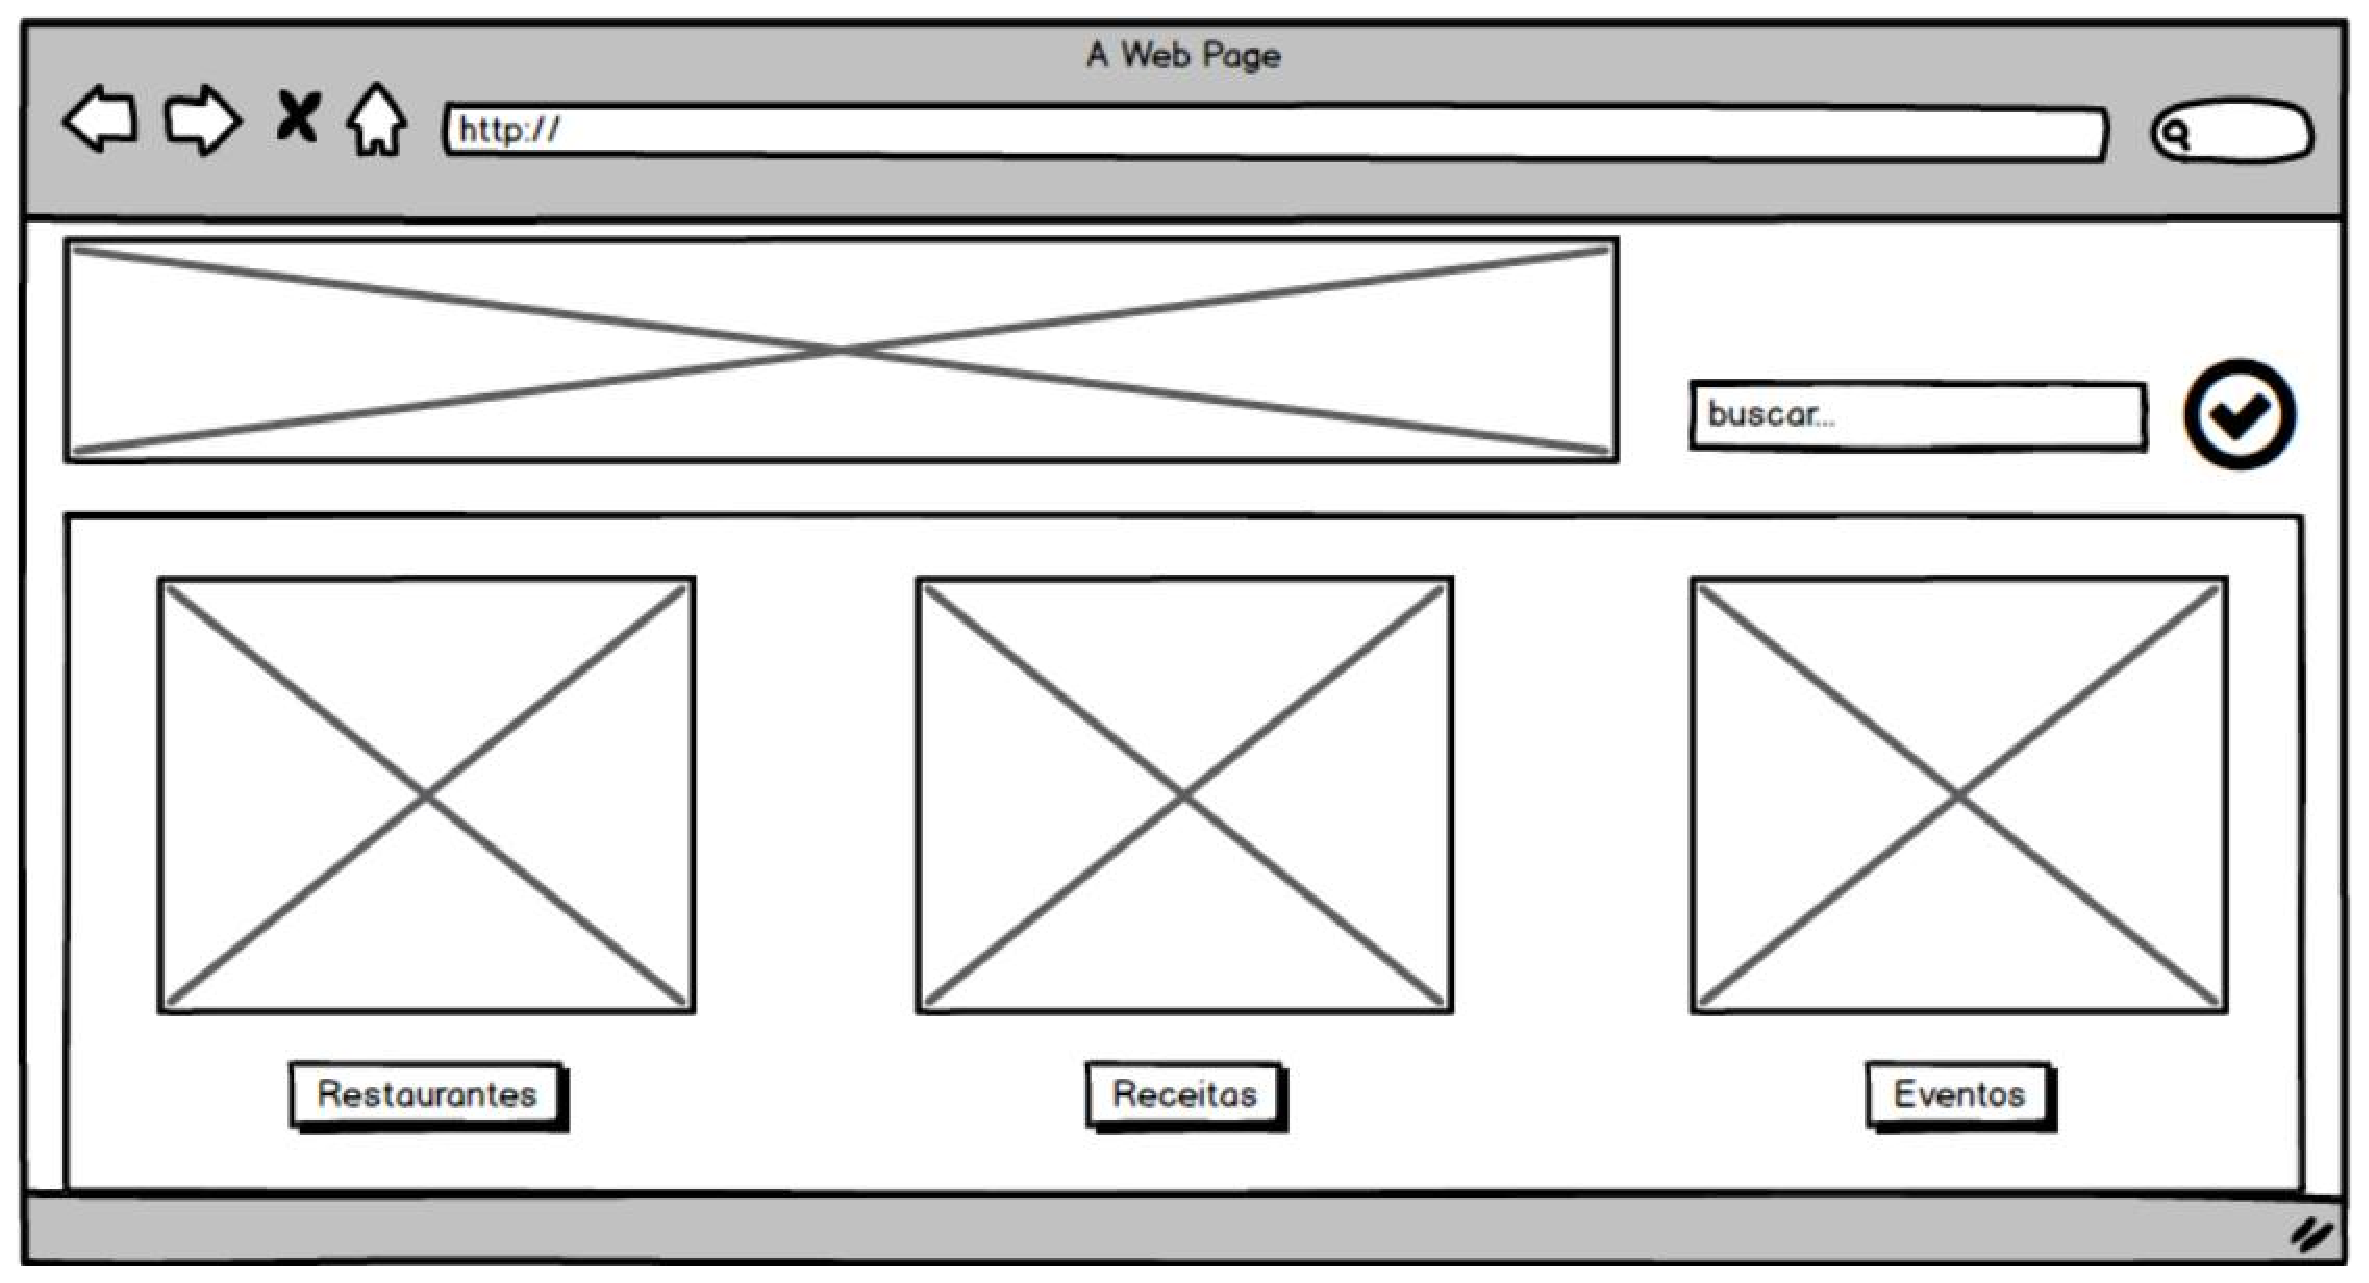
\includegraphics[keepaspectratio,scale=0.6]{figuras/media_fidelidade/prototipo1.eps}%
	\end{adjustbox}
\end{figure}

\begin{figure}[H]
	\begin{adjustbox}{
		addcode={
			\begin{minipage}{
				\width}}{
					\caption{Protótipo Média Fidelidade}
					\end{minipage}
				},
				rotate=90,center
			}
    	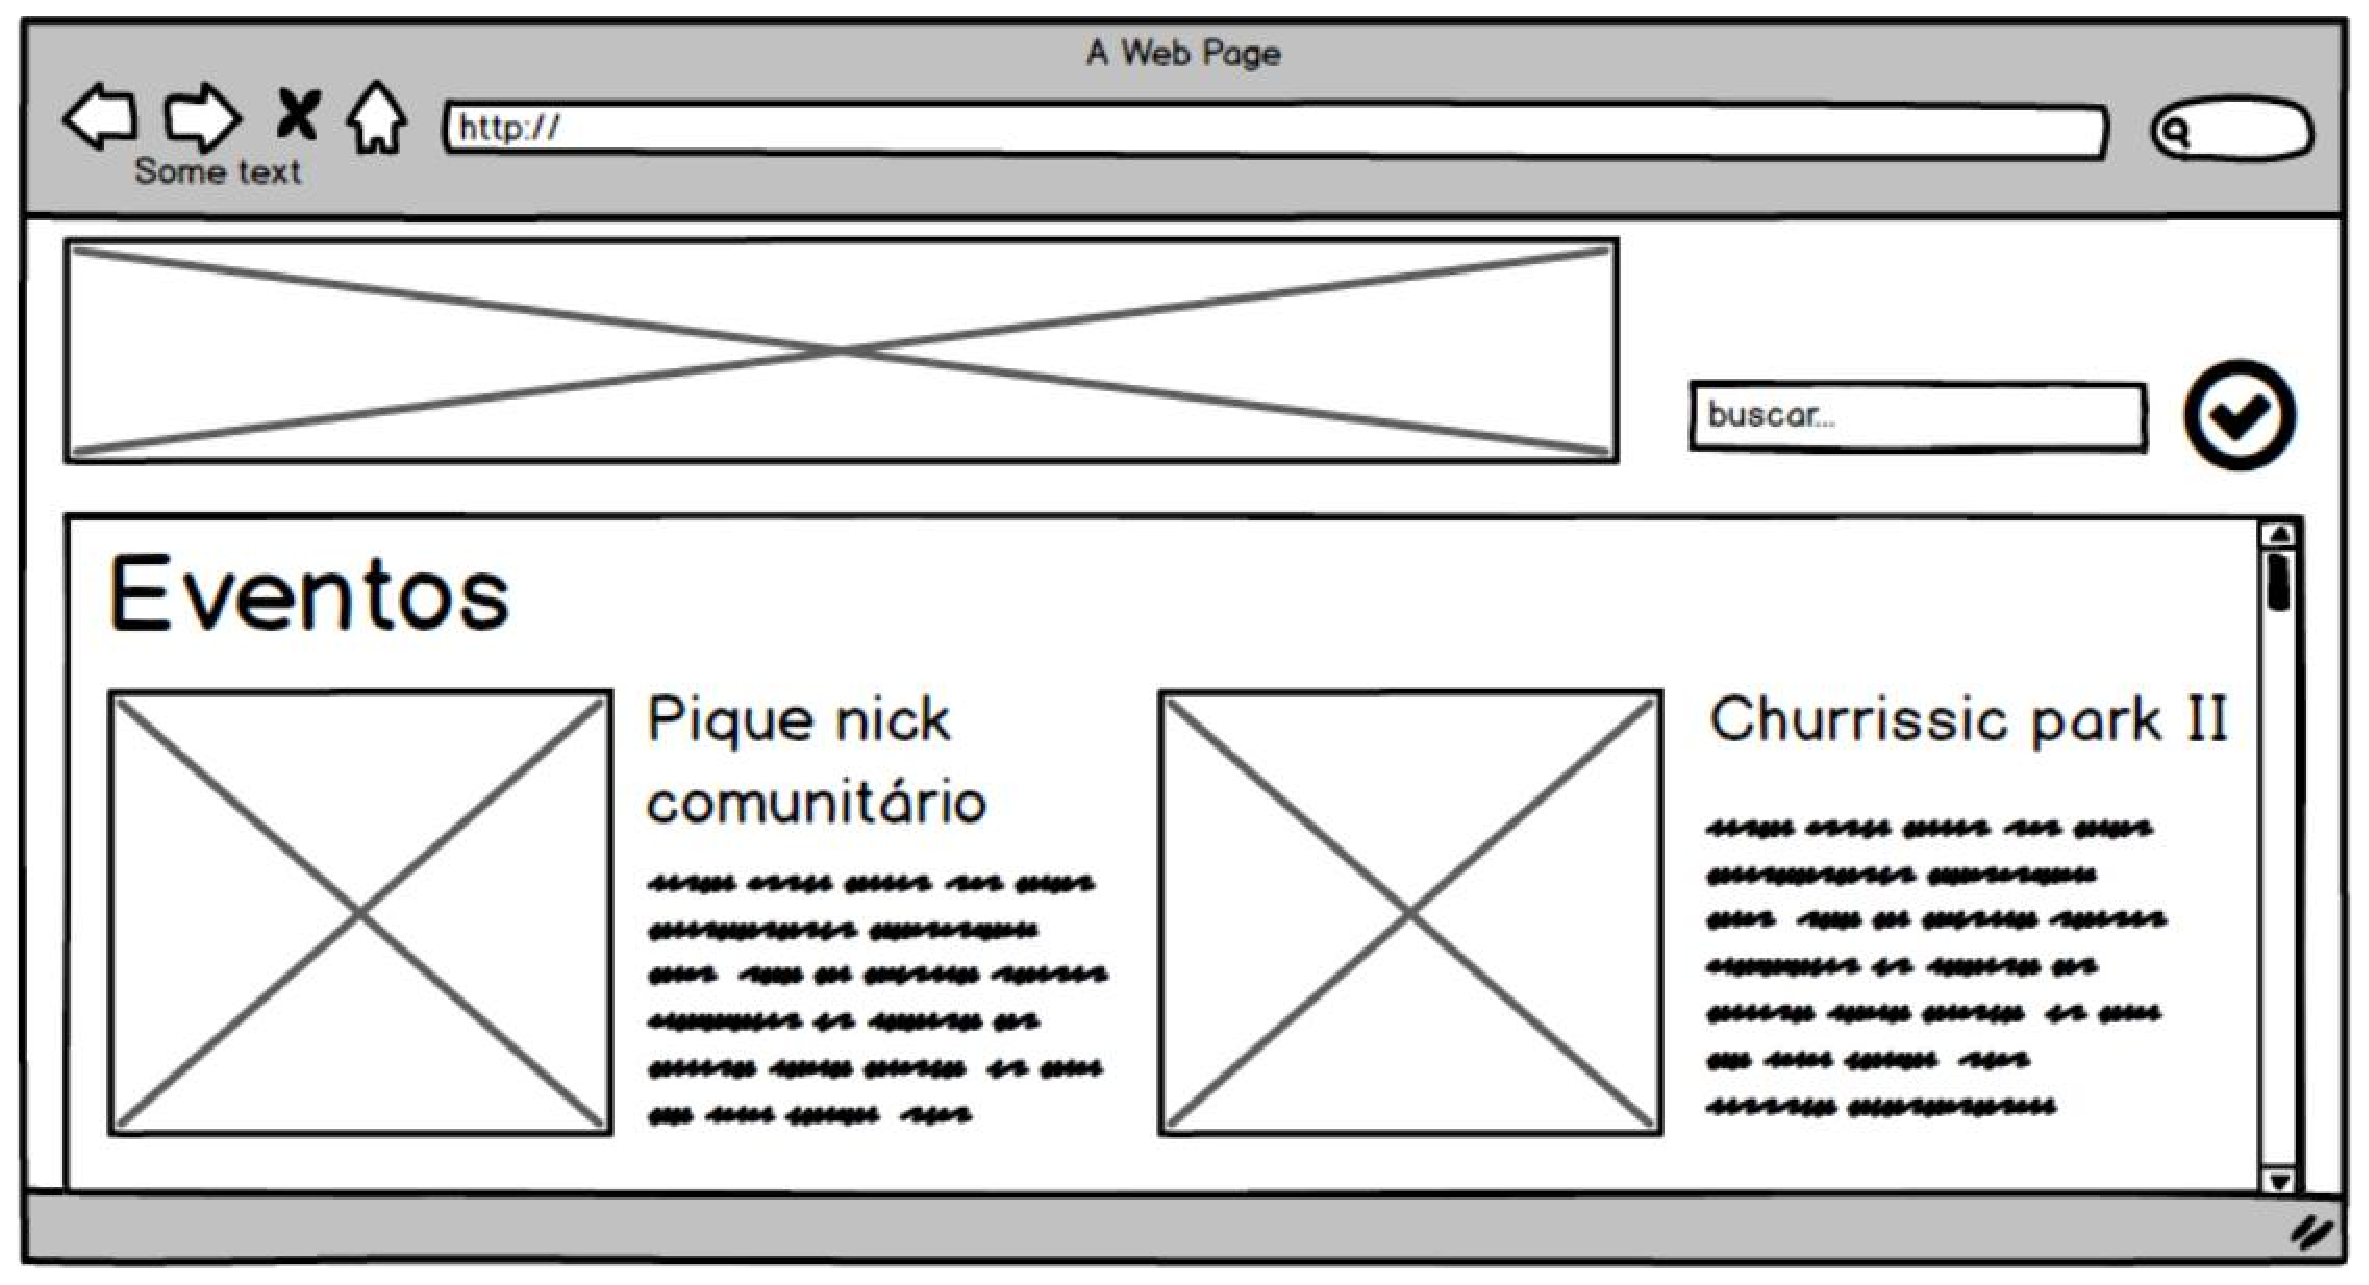
\includegraphics[keepaspectratio,scale=0.6]{figuras/media_fidelidade/prototipo2.eps}%
	\end{adjustbox}
\end{figure}

\begin{figure}[H]
	\begin{adjustbox}{
		addcode={
			\begin{minipage}{
				\width}}{
					\caption{Protótipo Média Fidelidade}
					\end{minipage}
				},
				rotate=90,center
			}
    	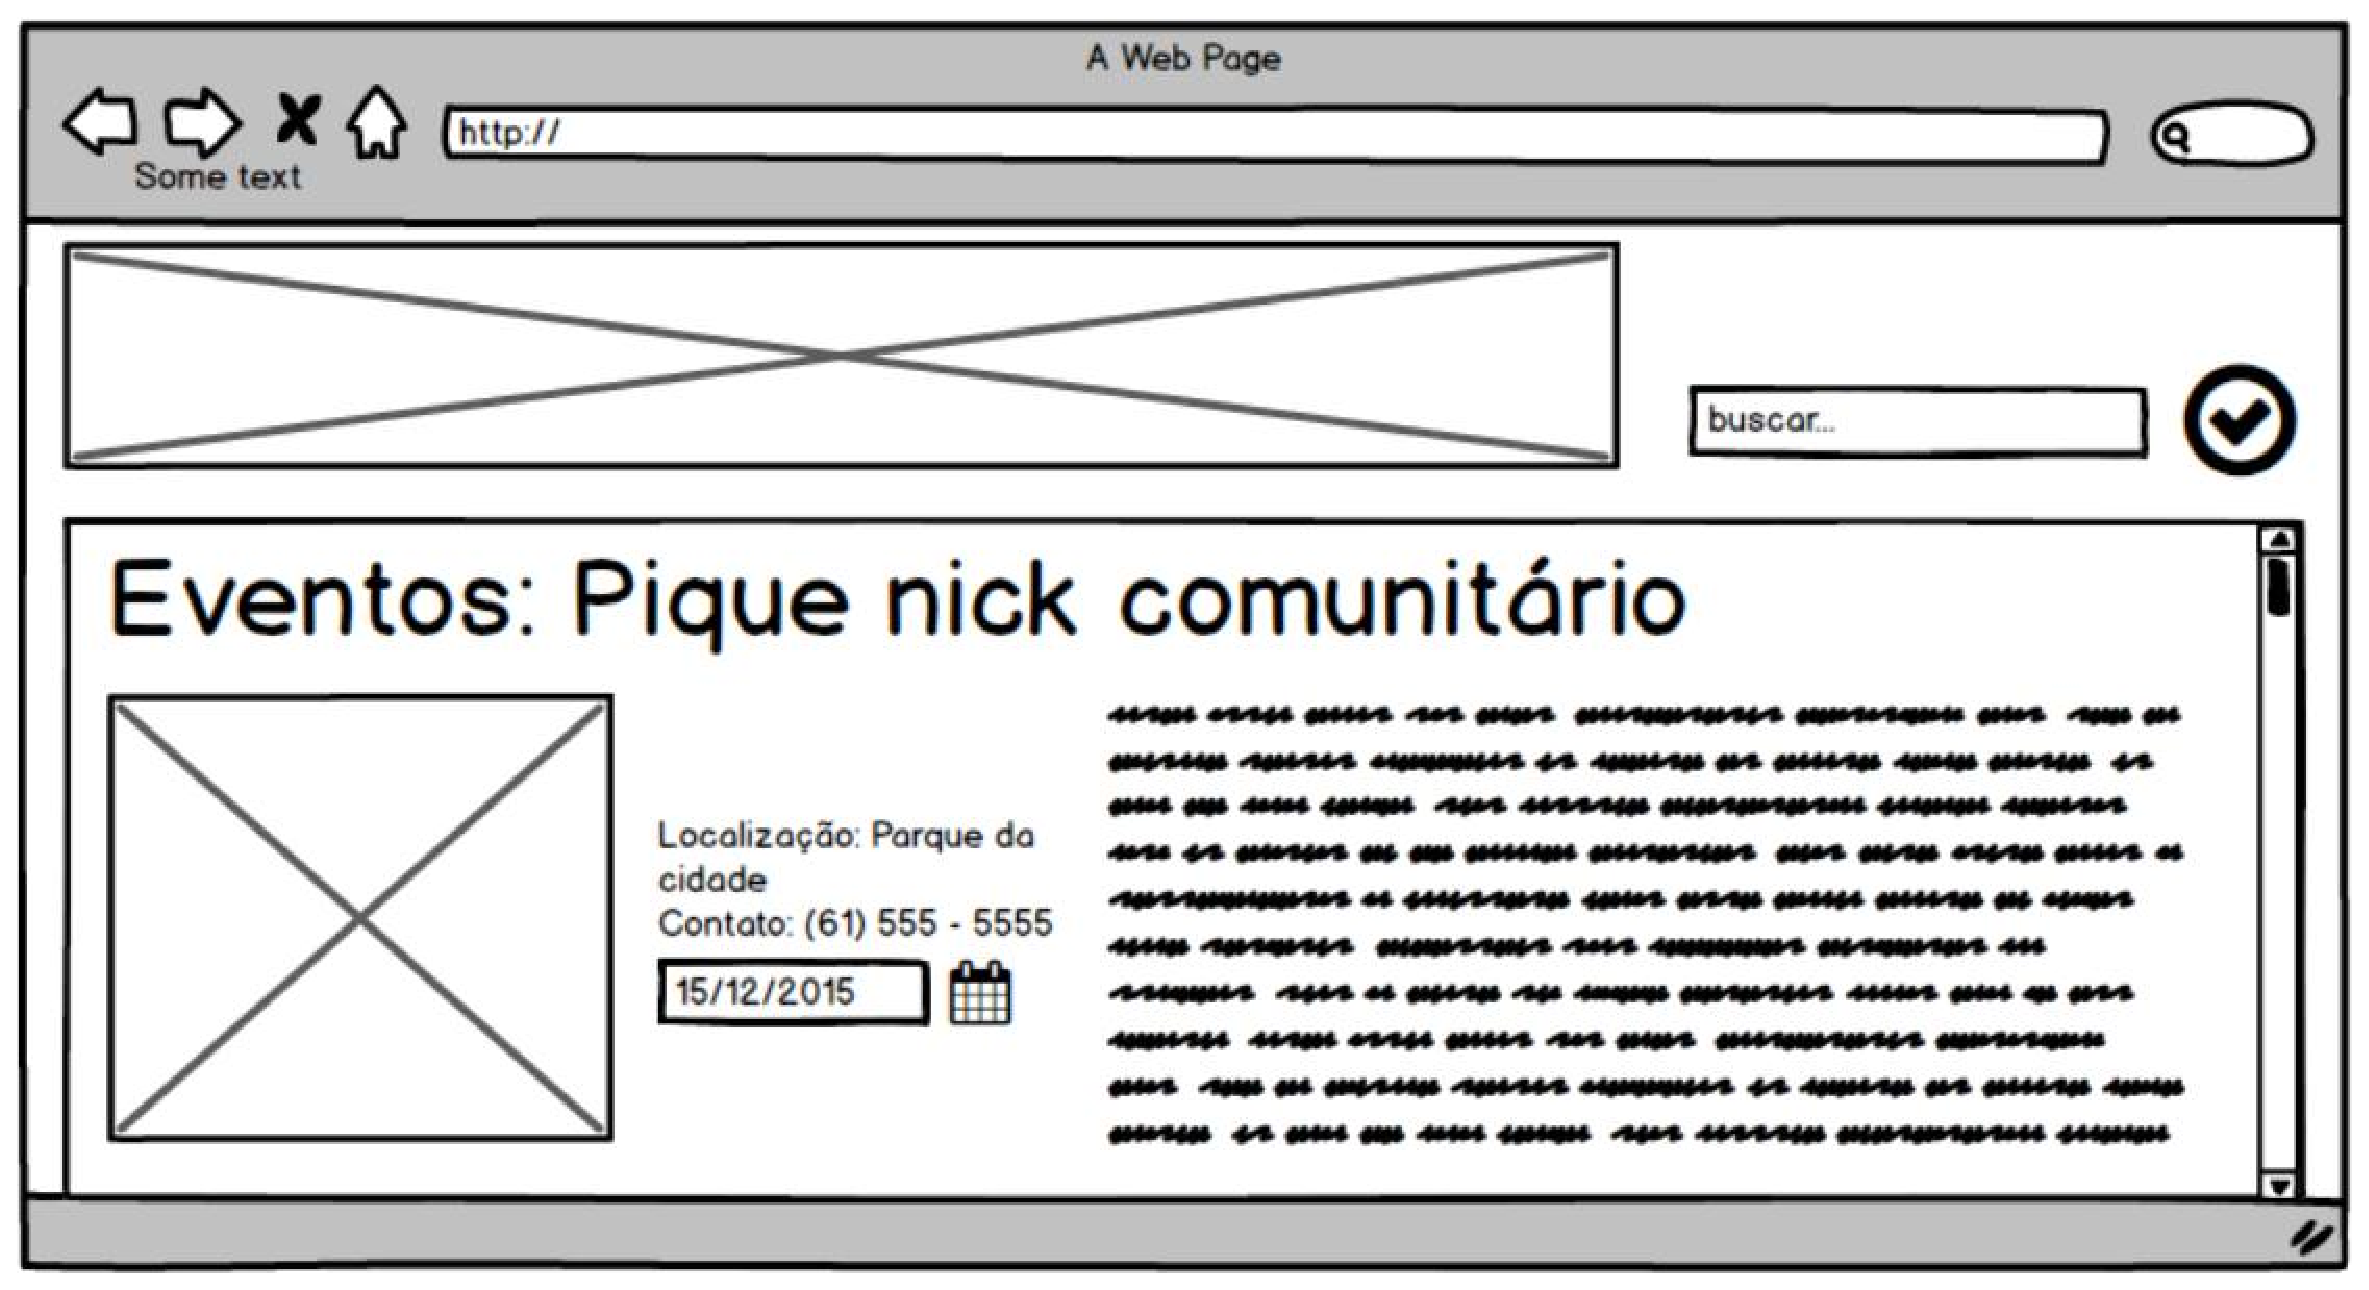
\includegraphics[keepaspectratio,scale=0.6]{figuras/media_fidelidade/prototipo3.eps}%
	\end{adjustbox}
\end{figure}

\begin{figure}[H]
	\begin{adjustbox}{
		addcode={
			\begin{minipage}{
				\width}}{
					\caption{Protótipo Média Fidelidade}
					\end{minipage}
				},
				rotate=90,center
			}
    	\includegraphics[keepaspectratio,scale=0.6]{figuras/media_fidelidade/prototipo4.eps}%
	\end{adjustbox}
\end{figure}

\begin{figure}[H]
	\begin{adjustbox}{
		addcode={
			\begin{minipage}{
				\width}}{
					\caption{Protótipo Média Fidelidade}
					\end{minipage}
				},
				rotate=90,center
			}
    	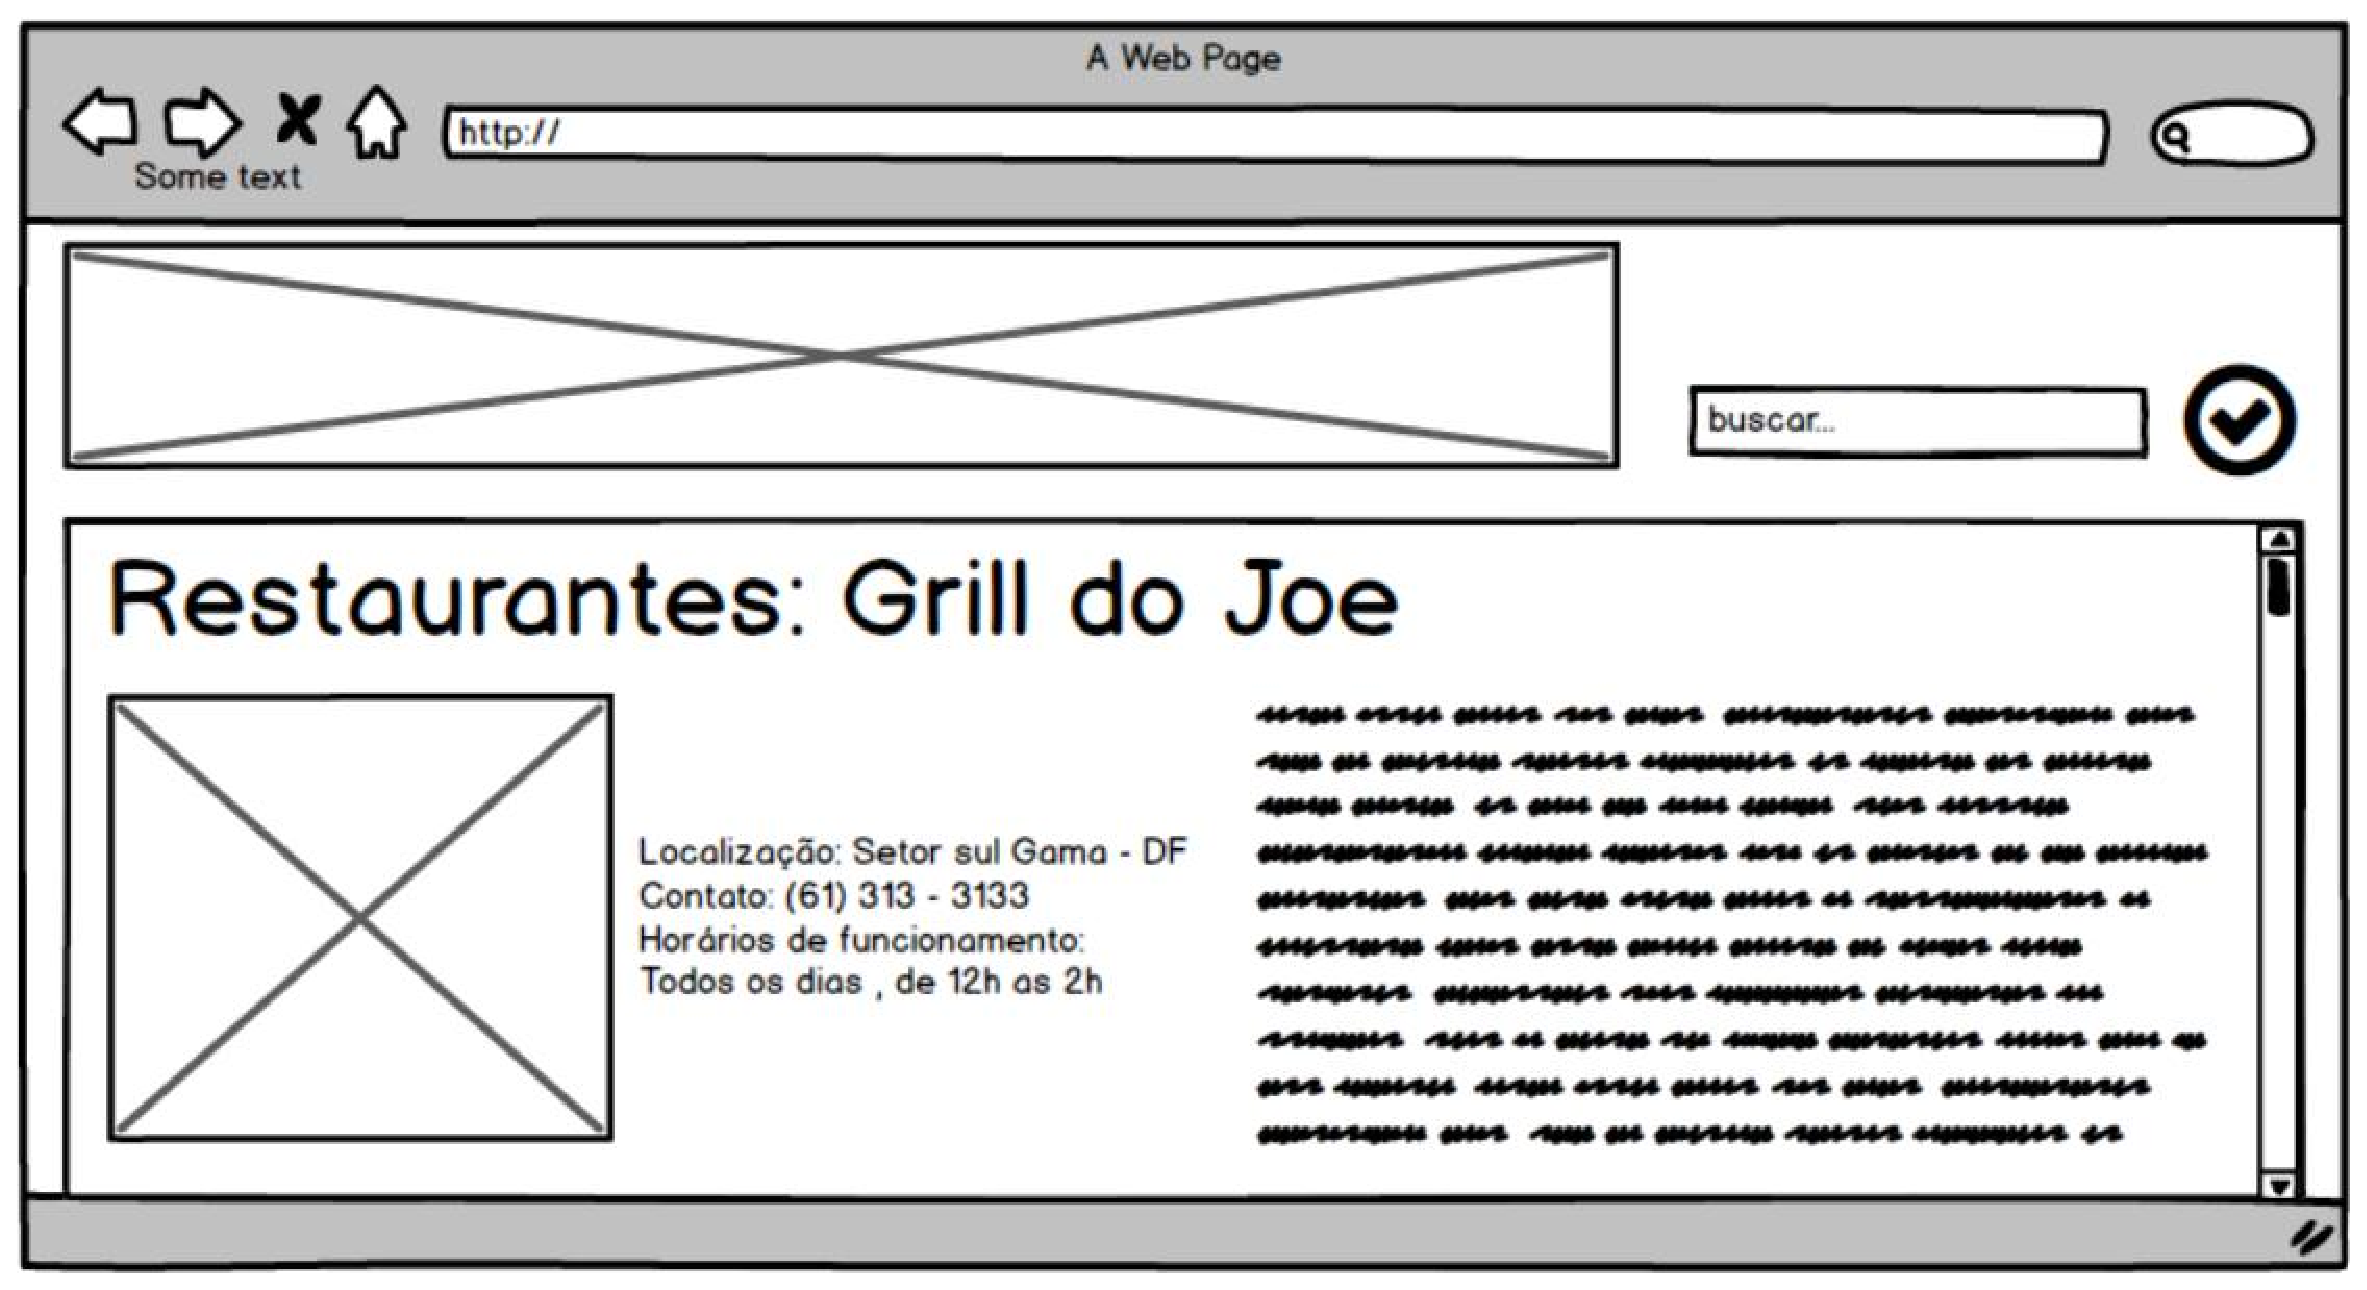
\includegraphics[keepaspectratio,scale=0.6]{figuras/media_fidelidade/prototipo5.eps}%
	\end{adjustbox}
\end{figure}

\begin{figure}[H]
	\begin{adjustbox}{
		addcode={
			\begin{minipage}{
				\width}}{
					\caption{Protótipo Média Fidelidade}
					\end{minipage}
				},
				rotate=90,center
			}
    	\includegraphics[keepaspectratio,scale=0.6]{figuras/media_fidelidade/prototipo6.eps}%
	\end{adjustbox}
\end{figure}

\begin{figure}[H]
	\begin{adjustbox}{
		addcode={
			\begin{minipage}{
				\width}}{
					\caption{Protótipo Média Fidelidade}
					\end{minipage}
				},
				rotate=90,center
			}
    	\includegraphics[keepaspectratio,scale=0.6]{figuras/media_fidelidade/prototipo7.eps}%
	\end{adjustbox}
\end{figure}

\section{Alta Fidelidade}

Os protótipos funcionais constituem a representação mais próxima do sistema que será desenvolvido. Nele é possível simular o fluxo completo das funcionalidades, permitindo a interação do usuário como se fosse o sistema final. A aparência visual, as formas de navegação e interatividade já são concebidas e aplicadas aos protótipos de alta fidelidade.

\textbf{Telas:}

\begin{figure}[H]
	\begin{adjustbox}{
		addcode={
			\begin{minipage}{
				\width}}{
					\caption{Protótipo Alta Fidelidade}
					\end{minipage}
				},
				rotate=90,center
			}
    	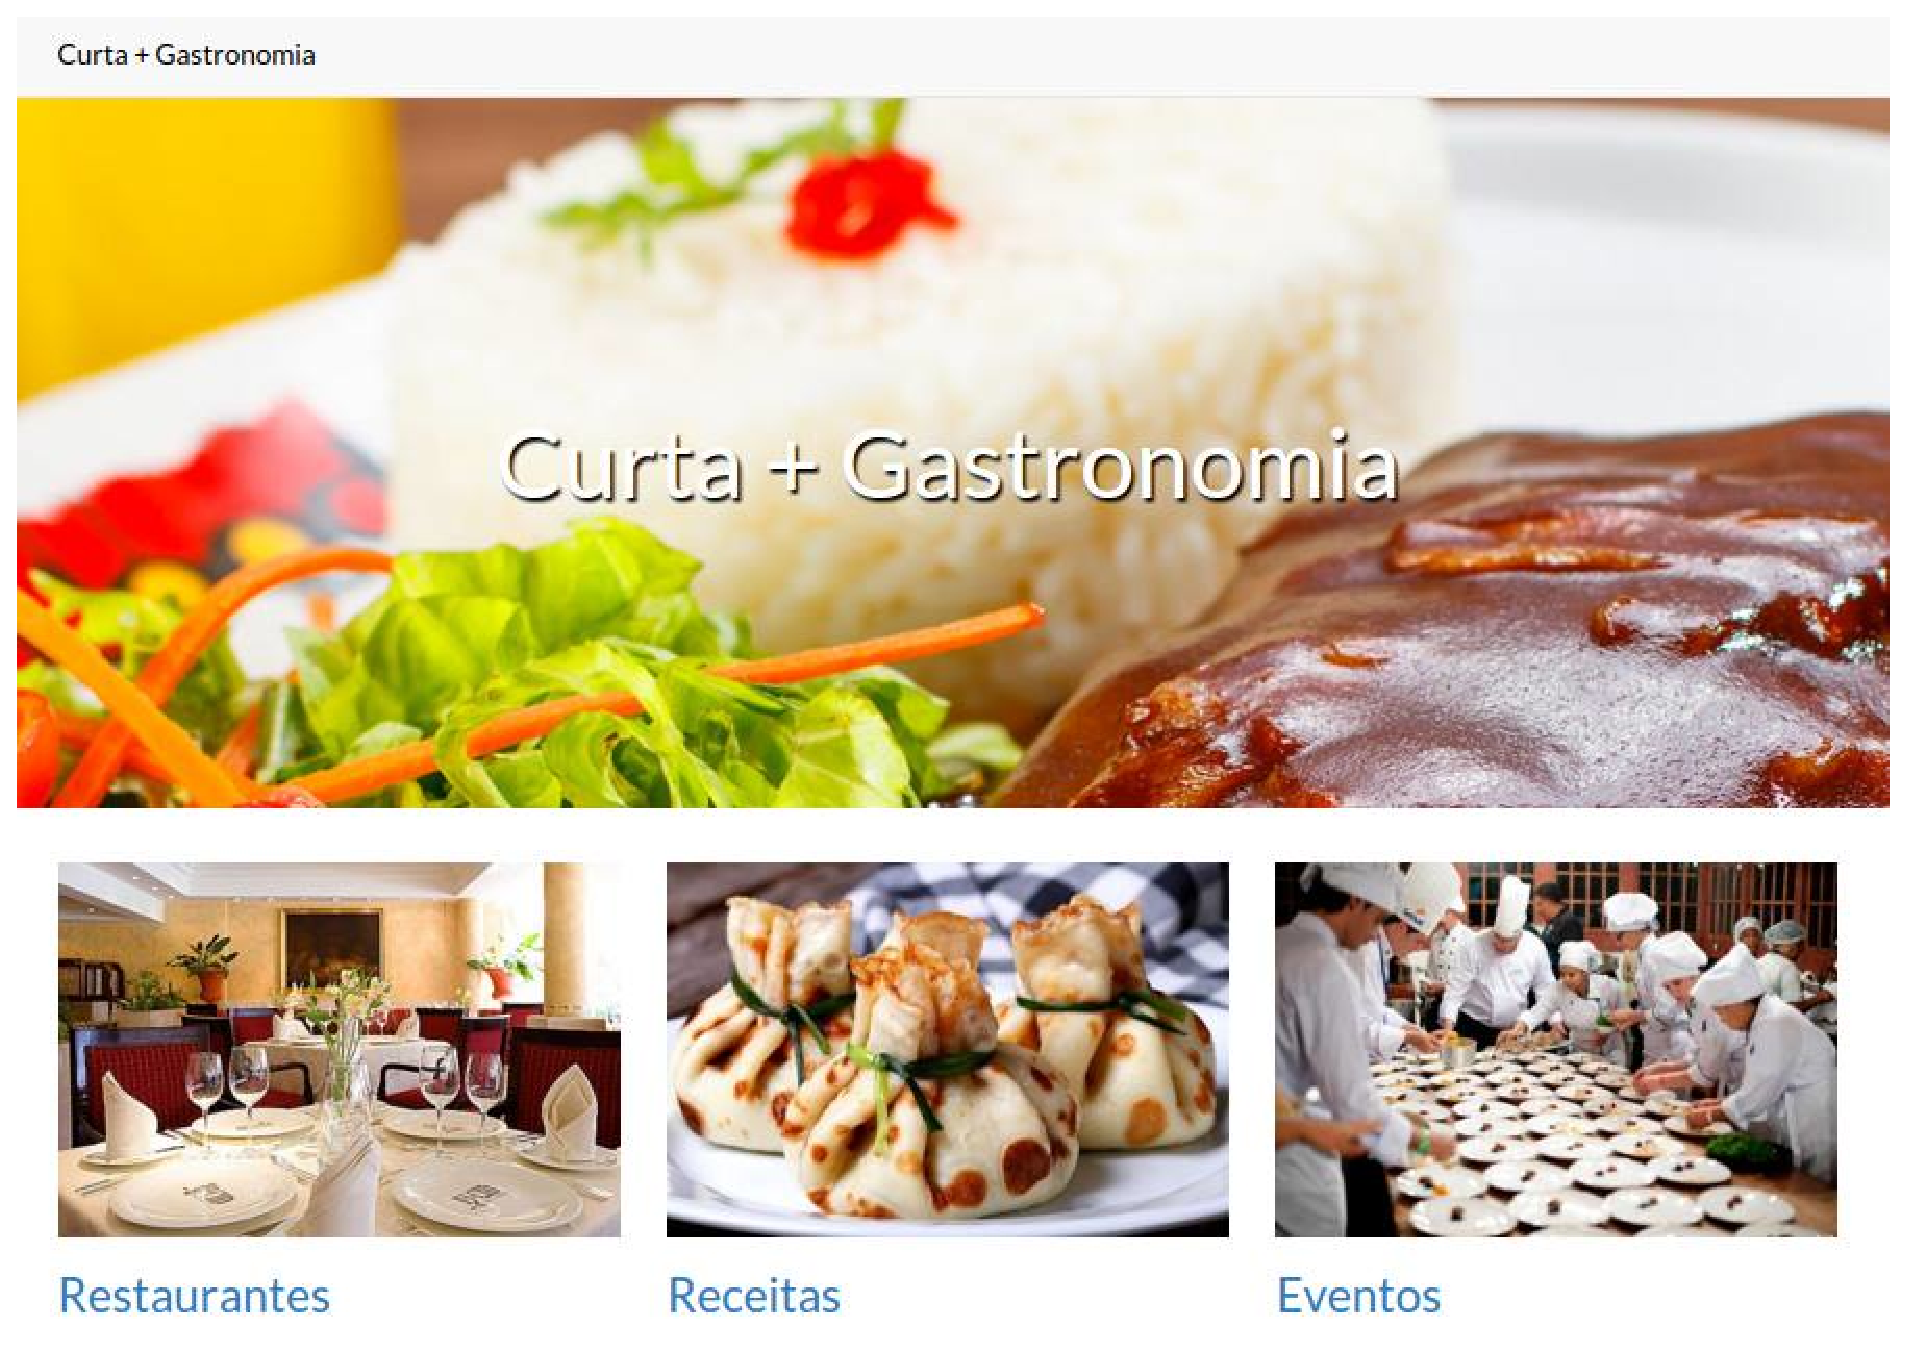
\includegraphics[keepaspectratio,scale=0.6]{figuras/alta_fidelidade/prototipo1.eps}%
	\end{adjustbox}
\end{figure}

\begin{figure}[H]
	\begin{adjustbox}{
		addcode={
			\begin{minipage}{
				\width}}{
					\caption{Protótipo Alta Fidelidade}
					\end{minipage}
				},
				rotate=90,center
			}
    	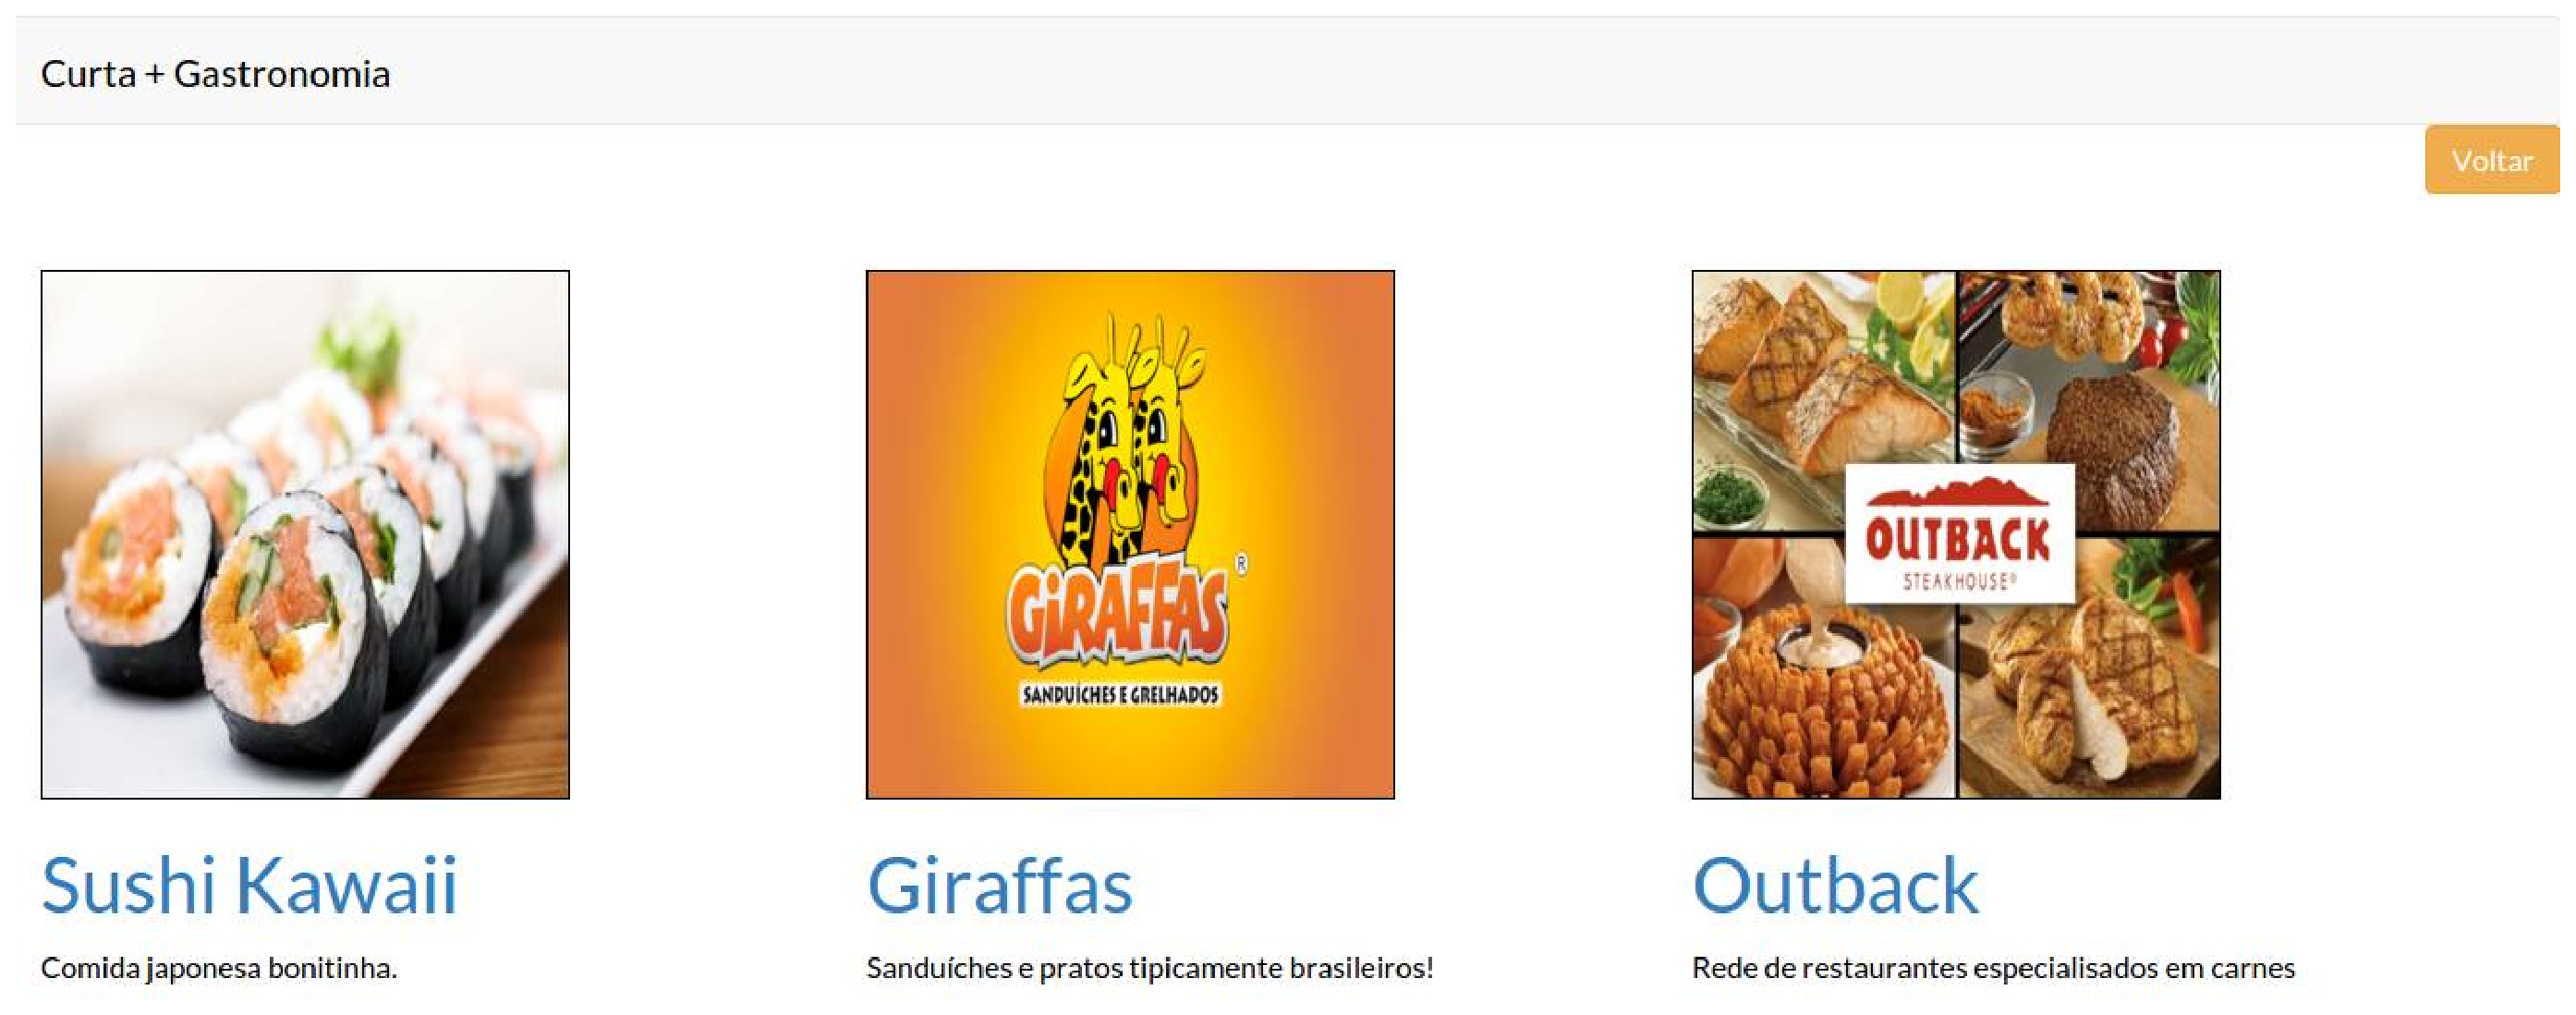
\includegraphics[keepaspectratio,scale=0.5]{figuras/alta_fidelidade/prototipo2.eps}%
	\end{adjustbox}
\end{figure}

\begin{figure}[H]
	\begin{adjustbox}{
		addcode={
			\begin{minipage}{
				\width}}{
					\caption{Protótipo Alta Fidelidade}
					\end{minipage}
				},
				rotate=90,center
			}
    	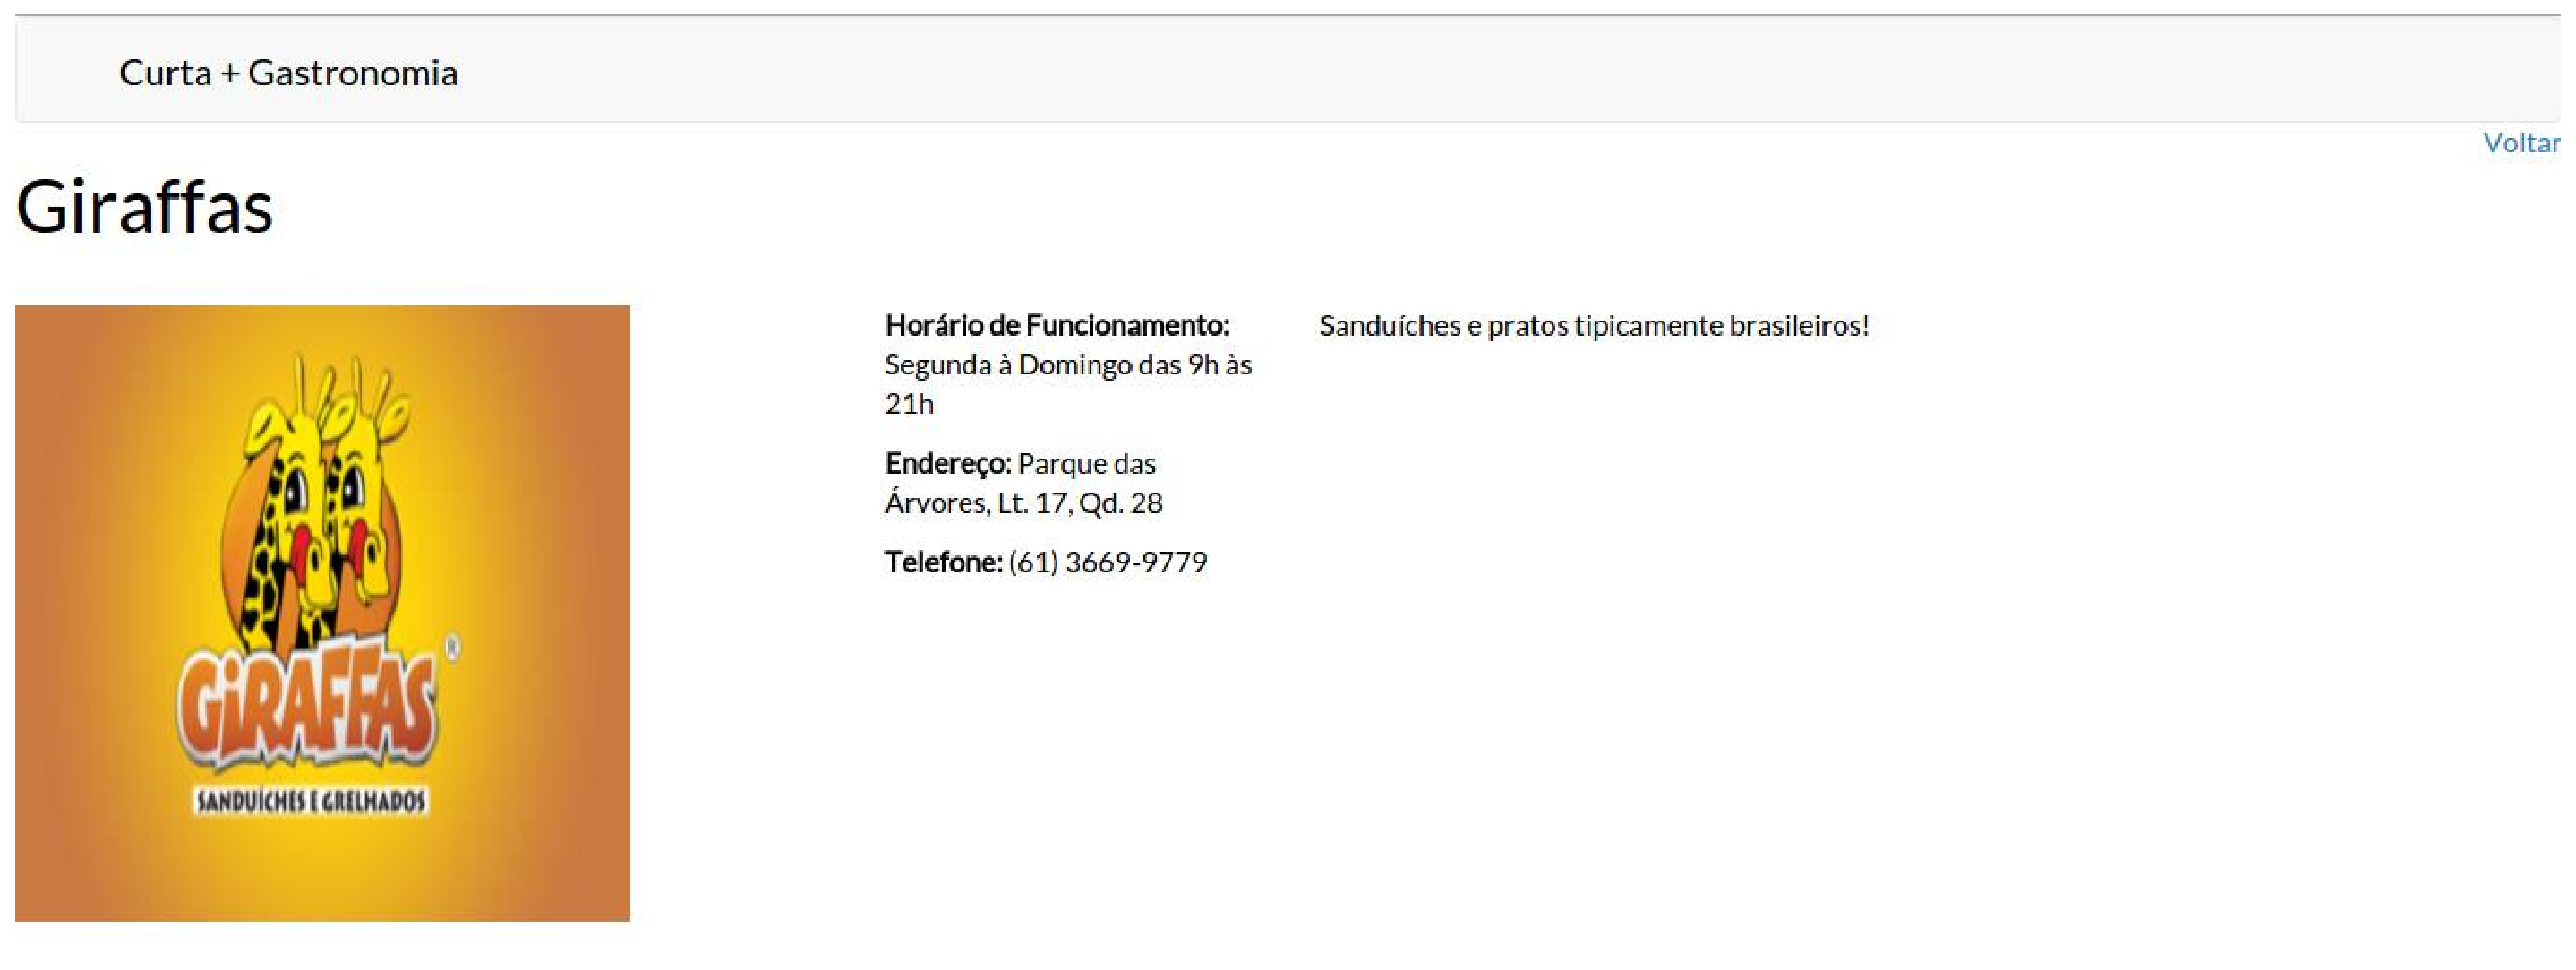
\includegraphics[keepaspectratio,scale=0.5]{figuras/alta_fidelidade/prototipo3.eps}%
	\end{adjustbox}
\end{figure}

\begin{figure}[H]
	\begin{adjustbox}{
		addcode={
			\begin{minipage}{
				\width}}{
					\caption{Protótipo Alta Fidelidade}
					\end{minipage}
				},
				rotate=90,center
			}
    	\includegraphics[keepaspectratio,scale=0.5]{figuras/alta_fidelidade/prototipo4.eps}%
	\end{adjustbox}
\end{figure}

\begin{figure}[H]
	\begin{adjustbox}{
		addcode={
			\begin{minipage}{
				\width}}{
					\caption{Protótipo Alta Fidelidade}
					\end{minipage}
				},
				rotate=90,center
			}
    	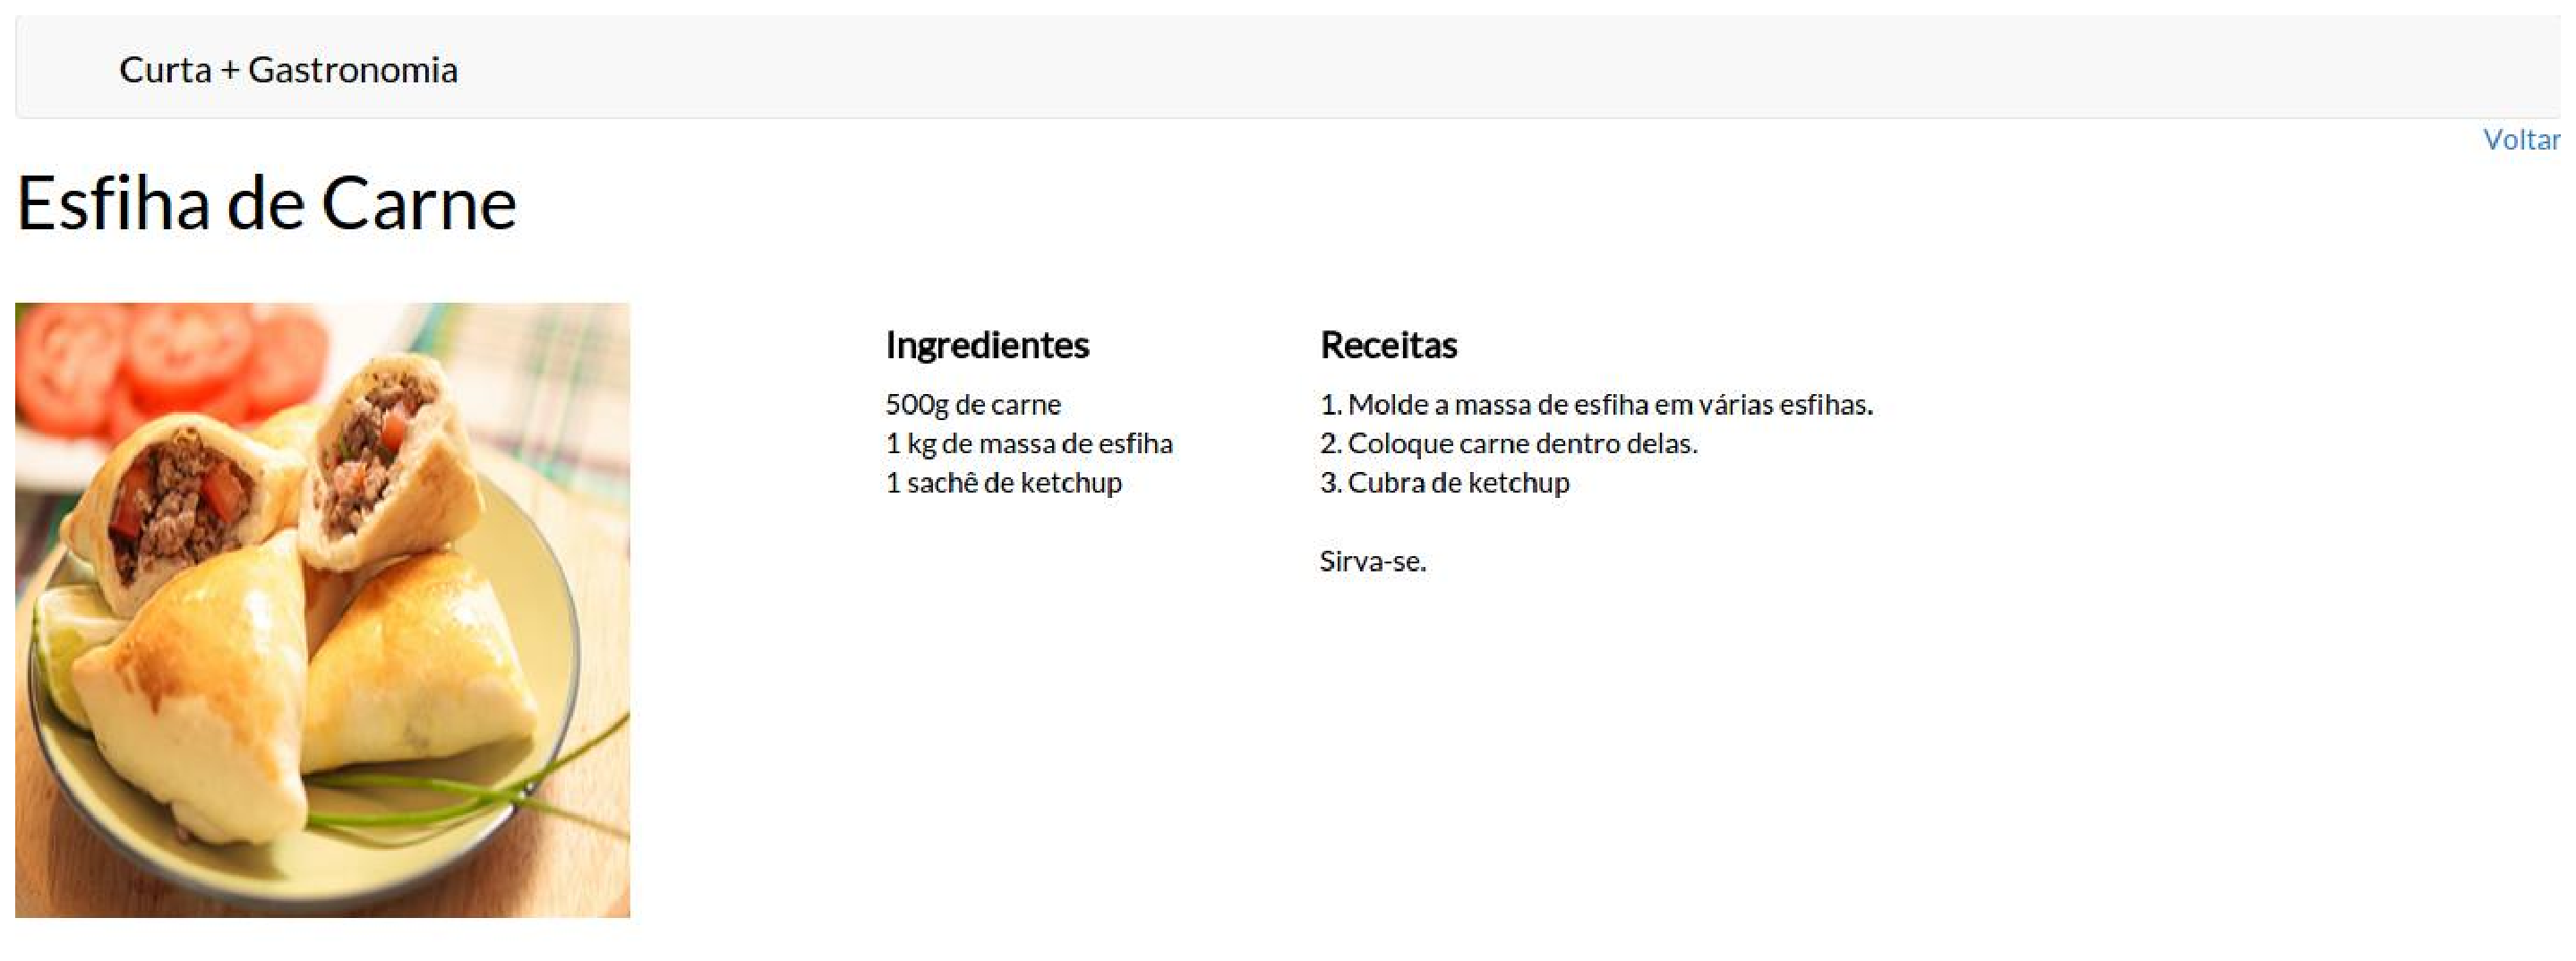
\includegraphics[keepaspectratio,scale=0.5]{figuras/alta_fidelidade/prototipo5.eps}%
	\end{adjustbox}
\end{figure}

\begin{figure}[H]
	\begin{adjustbox}{
		addcode={
			\begin{minipage}{
				\width}}{
					\caption{Protótipo Alta Fidelidade}
					\end{minipage}
				},
				rotate=90,center
			}
    	\includegraphics[keepaspectratio,scale=0.5]{figuras/alta_fidelidade/prototipo6.eps}%
	\end{adjustbox}
\end{figure}

\begin{figure}[H]
	\begin{adjustbox}{
		addcode={
			\begin{minipage}{
				\width}}{
					\caption{Protótipo Alta Fidelidade}
					\end{minipage}
				},
				rotate=90,center
			}
    	\includegraphics[keepaspectratio,scale=0.5]{figuras/alta_fidelidade/prototipo7.eps}%
	\end{adjustbox}
\end{figure}